\section{Práctica 1 - Instalación del entorno}

\subsection{Preparación del entorno}
    
Hemos preparado nuestro entorno de trabajo sobre Debian 7.8, versión de 32 bits\footnote{Inicialmente nuestra intención era trabajar sobre Debian 7.8 x64 pero tras problemas con Wine y No\$GBA decidimos usar la versión de 32 bits.}.
        
\subsubsection{Instalación de dependencias}

Antes de poder instalar el kit de herramientas para desarrollar para la Nintendo DS es necesario preparar el sistema para poder utilizar estas herramientas. Concretamente las dependencias del toolkit son {\tt make}, {\tt gcc} y {\tt tar}. El paquete {\tt desmume} es necesario si se quieren probar los proyectos usando el emulador  DeSmuME mientras que los paquetes {\tt wine} y {\tt unzip} son necesarios para poder emular el hardware objetivo mediante No\$GBA.

Esta última posibilidad es muy interesante ya que No\$GBA dispone de una versión especial orientada a facilitar en gran medida el desarrollo de software para la Nintendo DS e incluye, entre otras herramientas, un navegador de código ensamblador para poder saber qué instrucción está ejecutando la consola en cada momento y una consola de debug lo que permite imprimir mensajes desde la aplicación sin necesidad de interactuar con los controladores de las pantallas.

A pesar de no ser estrictamente necesario en nuestro caso hemos instalado algunas dependencias adicionales, entre ellas utilidades como {\tt wget} o {\tt g++}.
	
\begin{figure}[ht]
\begin{mdframed}[style=exampledefault]
\begin{verbatim}
sudo apt-get update -qy
sudo apt-get upgrade -qy
sudo apt-get install wget tar make gcc g++ desmume wine unzip \
    libc++6 libc6 -qy
\end{verbatim}
\end{mdframed}

	\caption{Los comandos ejecutados para instalar las dependencias en nuestro entorno de trabajo}
	\label{fig:installDependencies}
\end{figure}
	
\begin{figure}[h!]
	\caption{Resultados de la instalación de dependencias.}
	\label{fig:dependency}
	\centering
	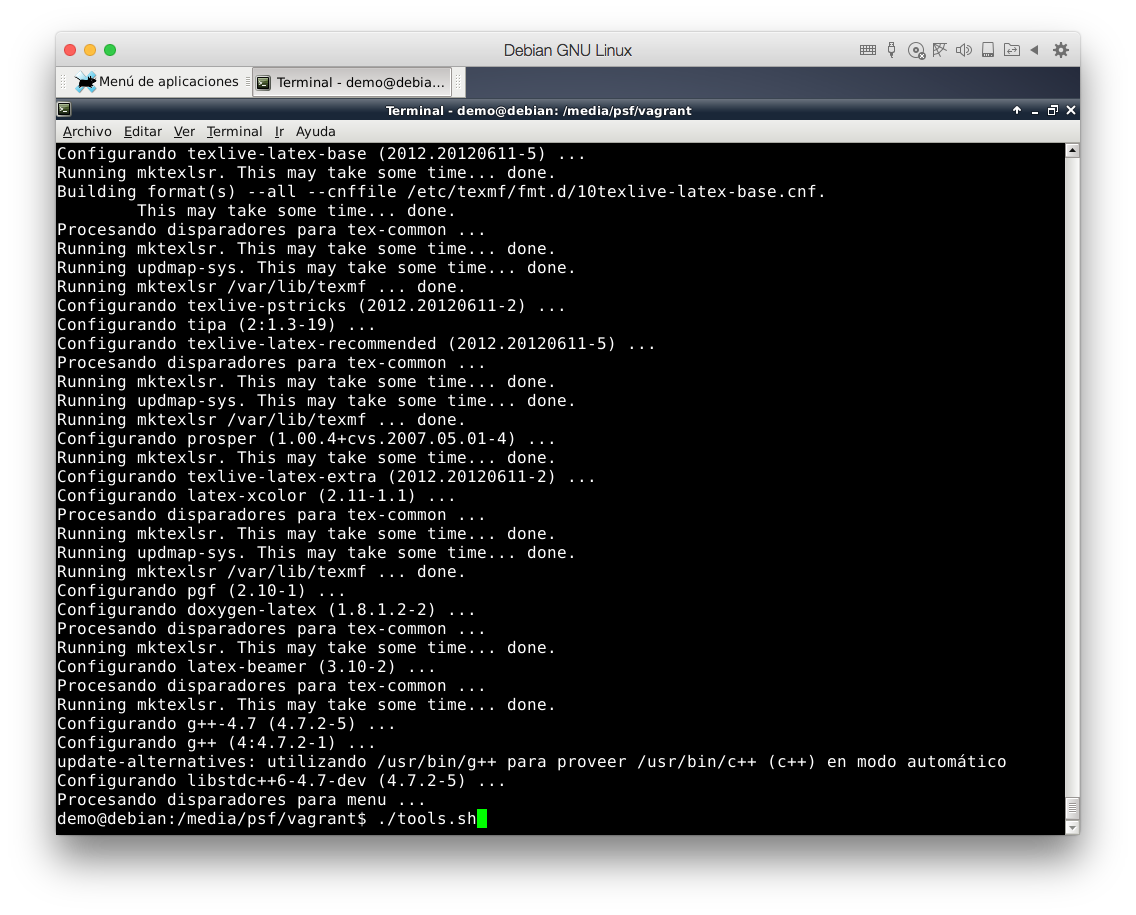
\includegraphics[width=0.95\textwidth]{P1Media/Dependencias}
\end{figure}
	
	\subsubsection{Instalación de las herramientas de desarrollo}
	
	Los pasos para la instalación de las herramientas de la guía de la práctica eran muy claros pero para facilitarnos la instalación de las herramientas en múltiples entornos de trabajo hemos agrupado todas las instrucciones en un único fichero para que instalar el kit de desarrollo fuese más sencillo.
	
	Este script (\textbf{Figura~\ref{fig:installToolkit}}) descarga {\tt devkitARM}, lo instala, prepara los archivos de configuración necesarios (realmente es tan sencillo como añadir un par de variables de entorno), descarga los ejemplos y los compila.
	
\begin{figure}[ht]
\begin{mdframed}[style=exampledefault]
\begin{verbatim}
cd ~/
wget -O ~/devkitARMupdate.pl http://goo.gl/rjbq5P
chmod a+x ~/devkitARMupdate.pl
~/devkitARMupdate.pl
export DEVKITPRO=~/devkitPro
export DEVKITARM=${DEVKITPRO}/devkitARM
echo "export DEVKITPRO=~/devkitPro" >>  ~/.bashrc
echo "export DEVKITARM=${DEVKITPRO}/devkitARM" >>  ~/.bashrc
echo "export DEVKITPRO=~/devkitPro" >>  ~/.zshrc
echo "export DEVKITARM=${DEVKITPRO}/devkitARM" >>  ~/.zshrc
wget -O /tmp/examples.tar.bz2 http://goo.gl/l5I1x1
tar xjvf /tmp/examples.tar.bz2
cd ~/devkitPro/examples/nds
make
cd ~/
wget -O gba.zip http://emuparadise.me/emulators/files/user/n-west-w-1776.zip
unzip gba.zip
\end{verbatim}
\end{mdframed}

	\caption{Los comandos ejecutados para instalar las herramientas de desarrollo y compilar los ejemplos}
	\label{fig:installToolkit}
\end{figure}

\begin{figure}[h!]
	\caption{Resultados de la instalación del toolkit.}
	\label{fig:dependency}
	\centering
	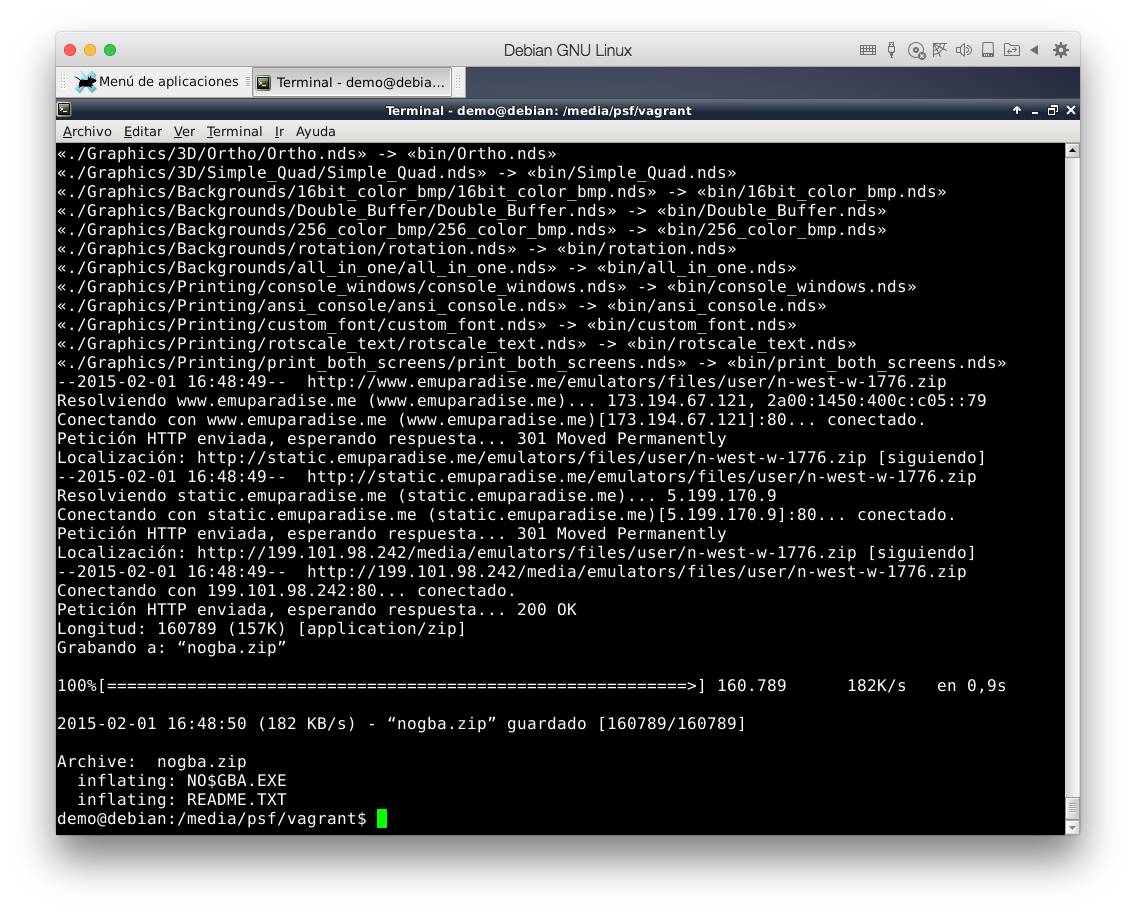
\includegraphics[width=0.95\textwidth]{P1Media/Toolkit}
\end{figure}

	Nótese que este script no siempre funcionará de forma automática: algunos los enlaces usados son los enlaces de descarga directa temporales de {\tt SourceForge.net}, que expiran tras cierto tiempo. Cuando expiran es necesario esperar unos segundos para descargar el fichero y es posible que el script lo que descargue sean las páginas de espera en lugar de los ficheros deseados. La solución es simple: basta con acceder al link de descarga caducado mediante un navegador web y extraer el nuevo link de descarga inmediata (aparece bajo el título ``direct link'').
	
	\newpage
	
	\subsection{Ejecución}
	
	\subsubsection{Compilación de los proyectos de prueba}
	
	Los proyectos de prueba pueden compilarse tanto mediante el comando {\tt make} ejecutado en la raíz de la carpeta que contiene los programas de ejemplo como mediante el mismo comando {\tt make} ejecutado en la carpeta de cada proyecto. La diferencia radica en que mediante el primer método se compilan todas las aplicaciones de ejemplo mientras que la segunda opción únicamente compila un proyecto concreto, dependiendo de las necesidades de cada momento convendrá usar una aproximación u otra.
	
\begin{figure}[h!]
	\caption{Resultados de la compilación del proyecto {\tt Hello World}.}
	\label{fig:dependency}
	\centering
	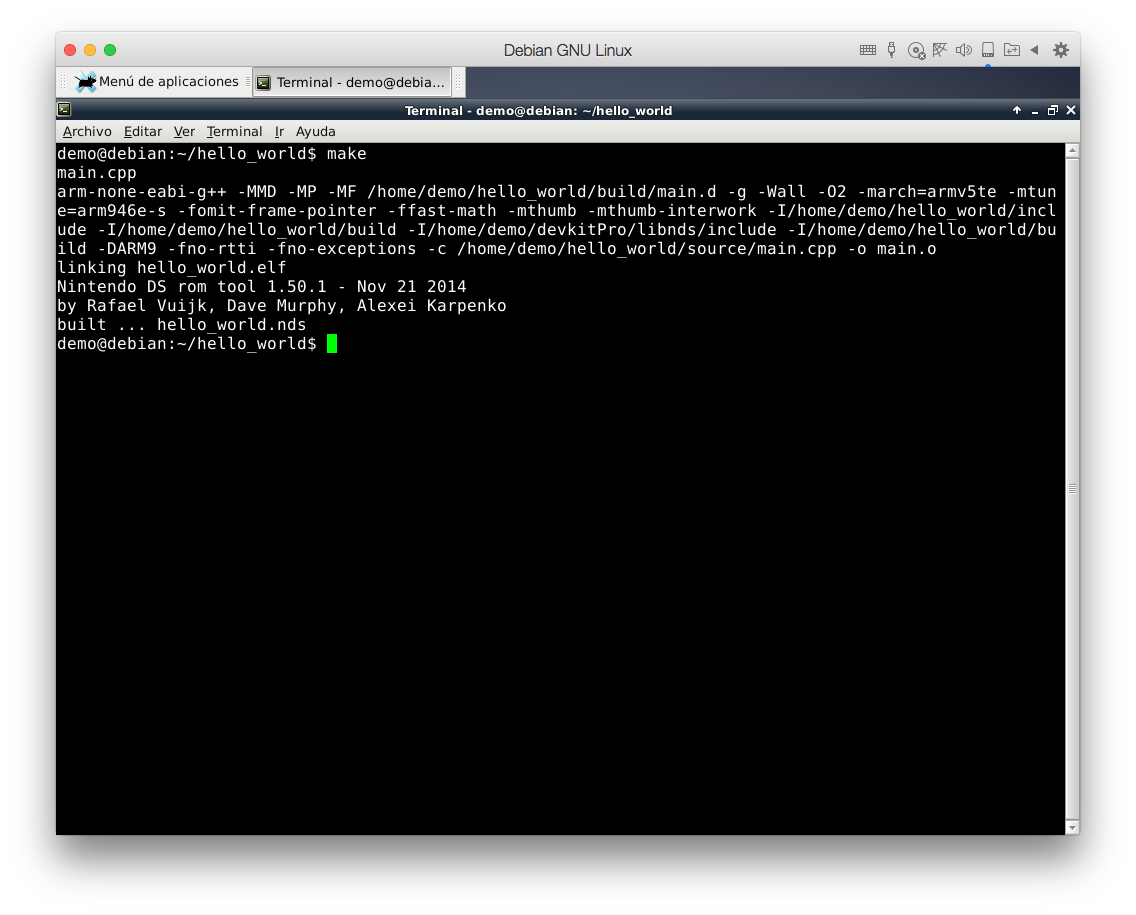
\includegraphics[width=0.95\textwidth]{P1Media/Compilado}
\end{figure}
	
	\subsubsection{Emulación de los proyectos de prueba}
	
	El emulador DeSmuME puede ser invocado desde la terminal mediante el comando {\tt desmume <ruta a fichero .nds>}, sin embargo No\$GBA no acepta ningún argumento, además requiere ser invocado mediante {\tt wine} por lo que en nuestro entorno hemos dispuesto de los siguientes alias:
	
\begin{figure}[ht]
\begin{mdframed}[style=exampledefault]
\begin{verbatim}
alias nocashgba="wine ~/NOcashGBA.exe"
alias nocashgbadebug="wine ~/NOcashGBAdebug.exe"
\end{verbatim}
\end{mdframed}

	\caption{Alias para ejecutar No\$GBA más cómodamente.}
	\label{fig:nocashAlias}
\end{figure}
	
\begin{figure}[h!]
	\caption{{\tt Hello World} ejecutado en {\tt DeSmuME}.}
	\label{fig:dependency}
	\centering
	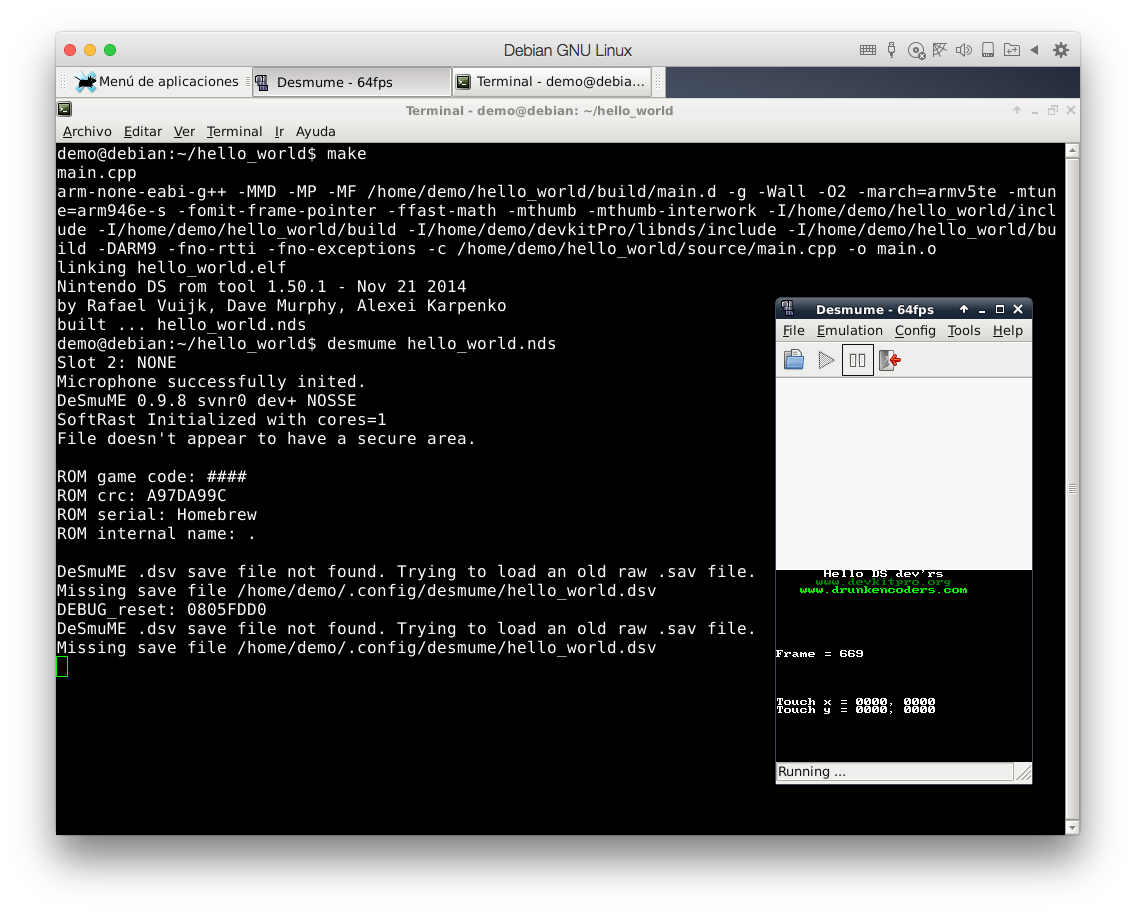
\includegraphics[width=0.95\textwidth]{P1Media/DeSmuME}
\end{figure}
	
\begin{figure}[h!]
	\caption{{\tt Hello World} ejecutado en {\tt No\$GBA}.}
	\label{fig:dependency}
	\centering
	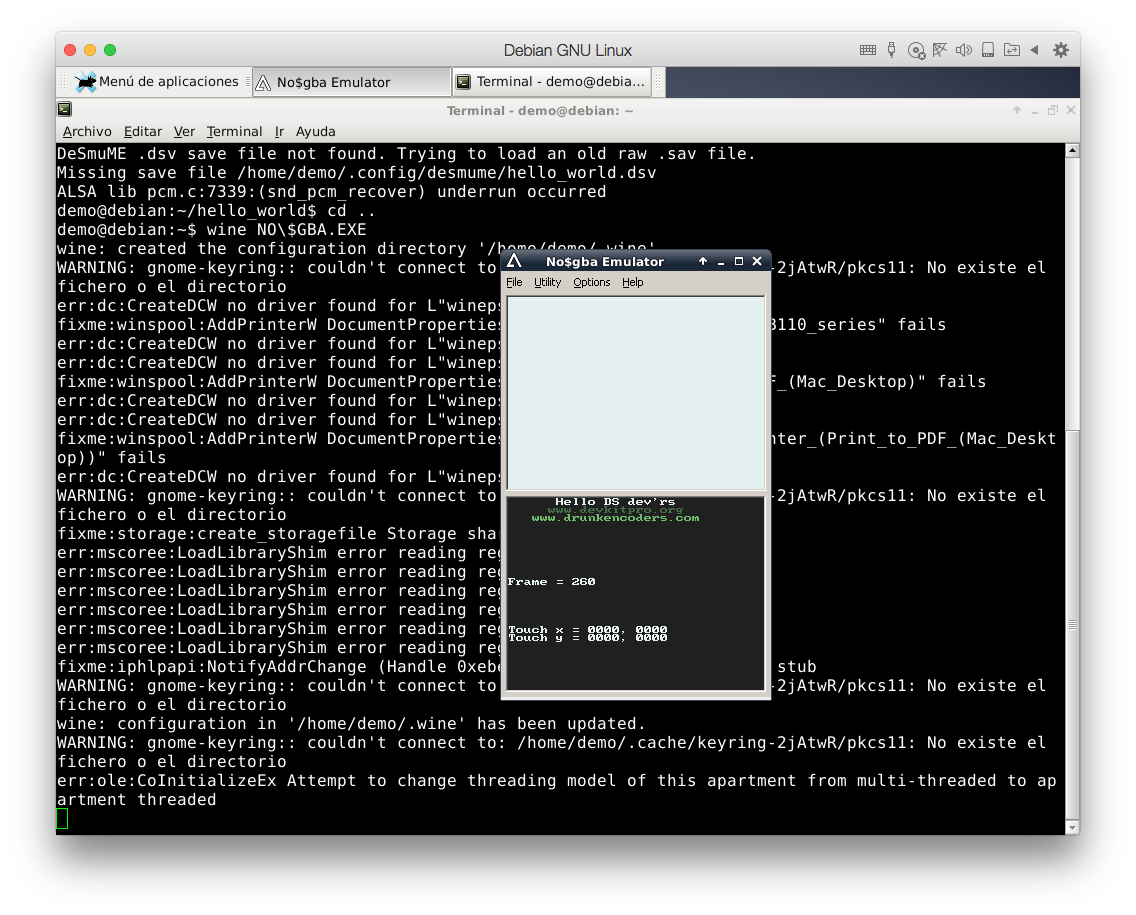
\includegraphics[width=0.95\textwidth]{P1Media/NoCash}
\end{figure}

\begin{figure}[h!]
	\caption{{\tt Hello World} ejecutado en {\tt No\$GBA} debugger.}
	\label{fig:dependency}
	\centering
	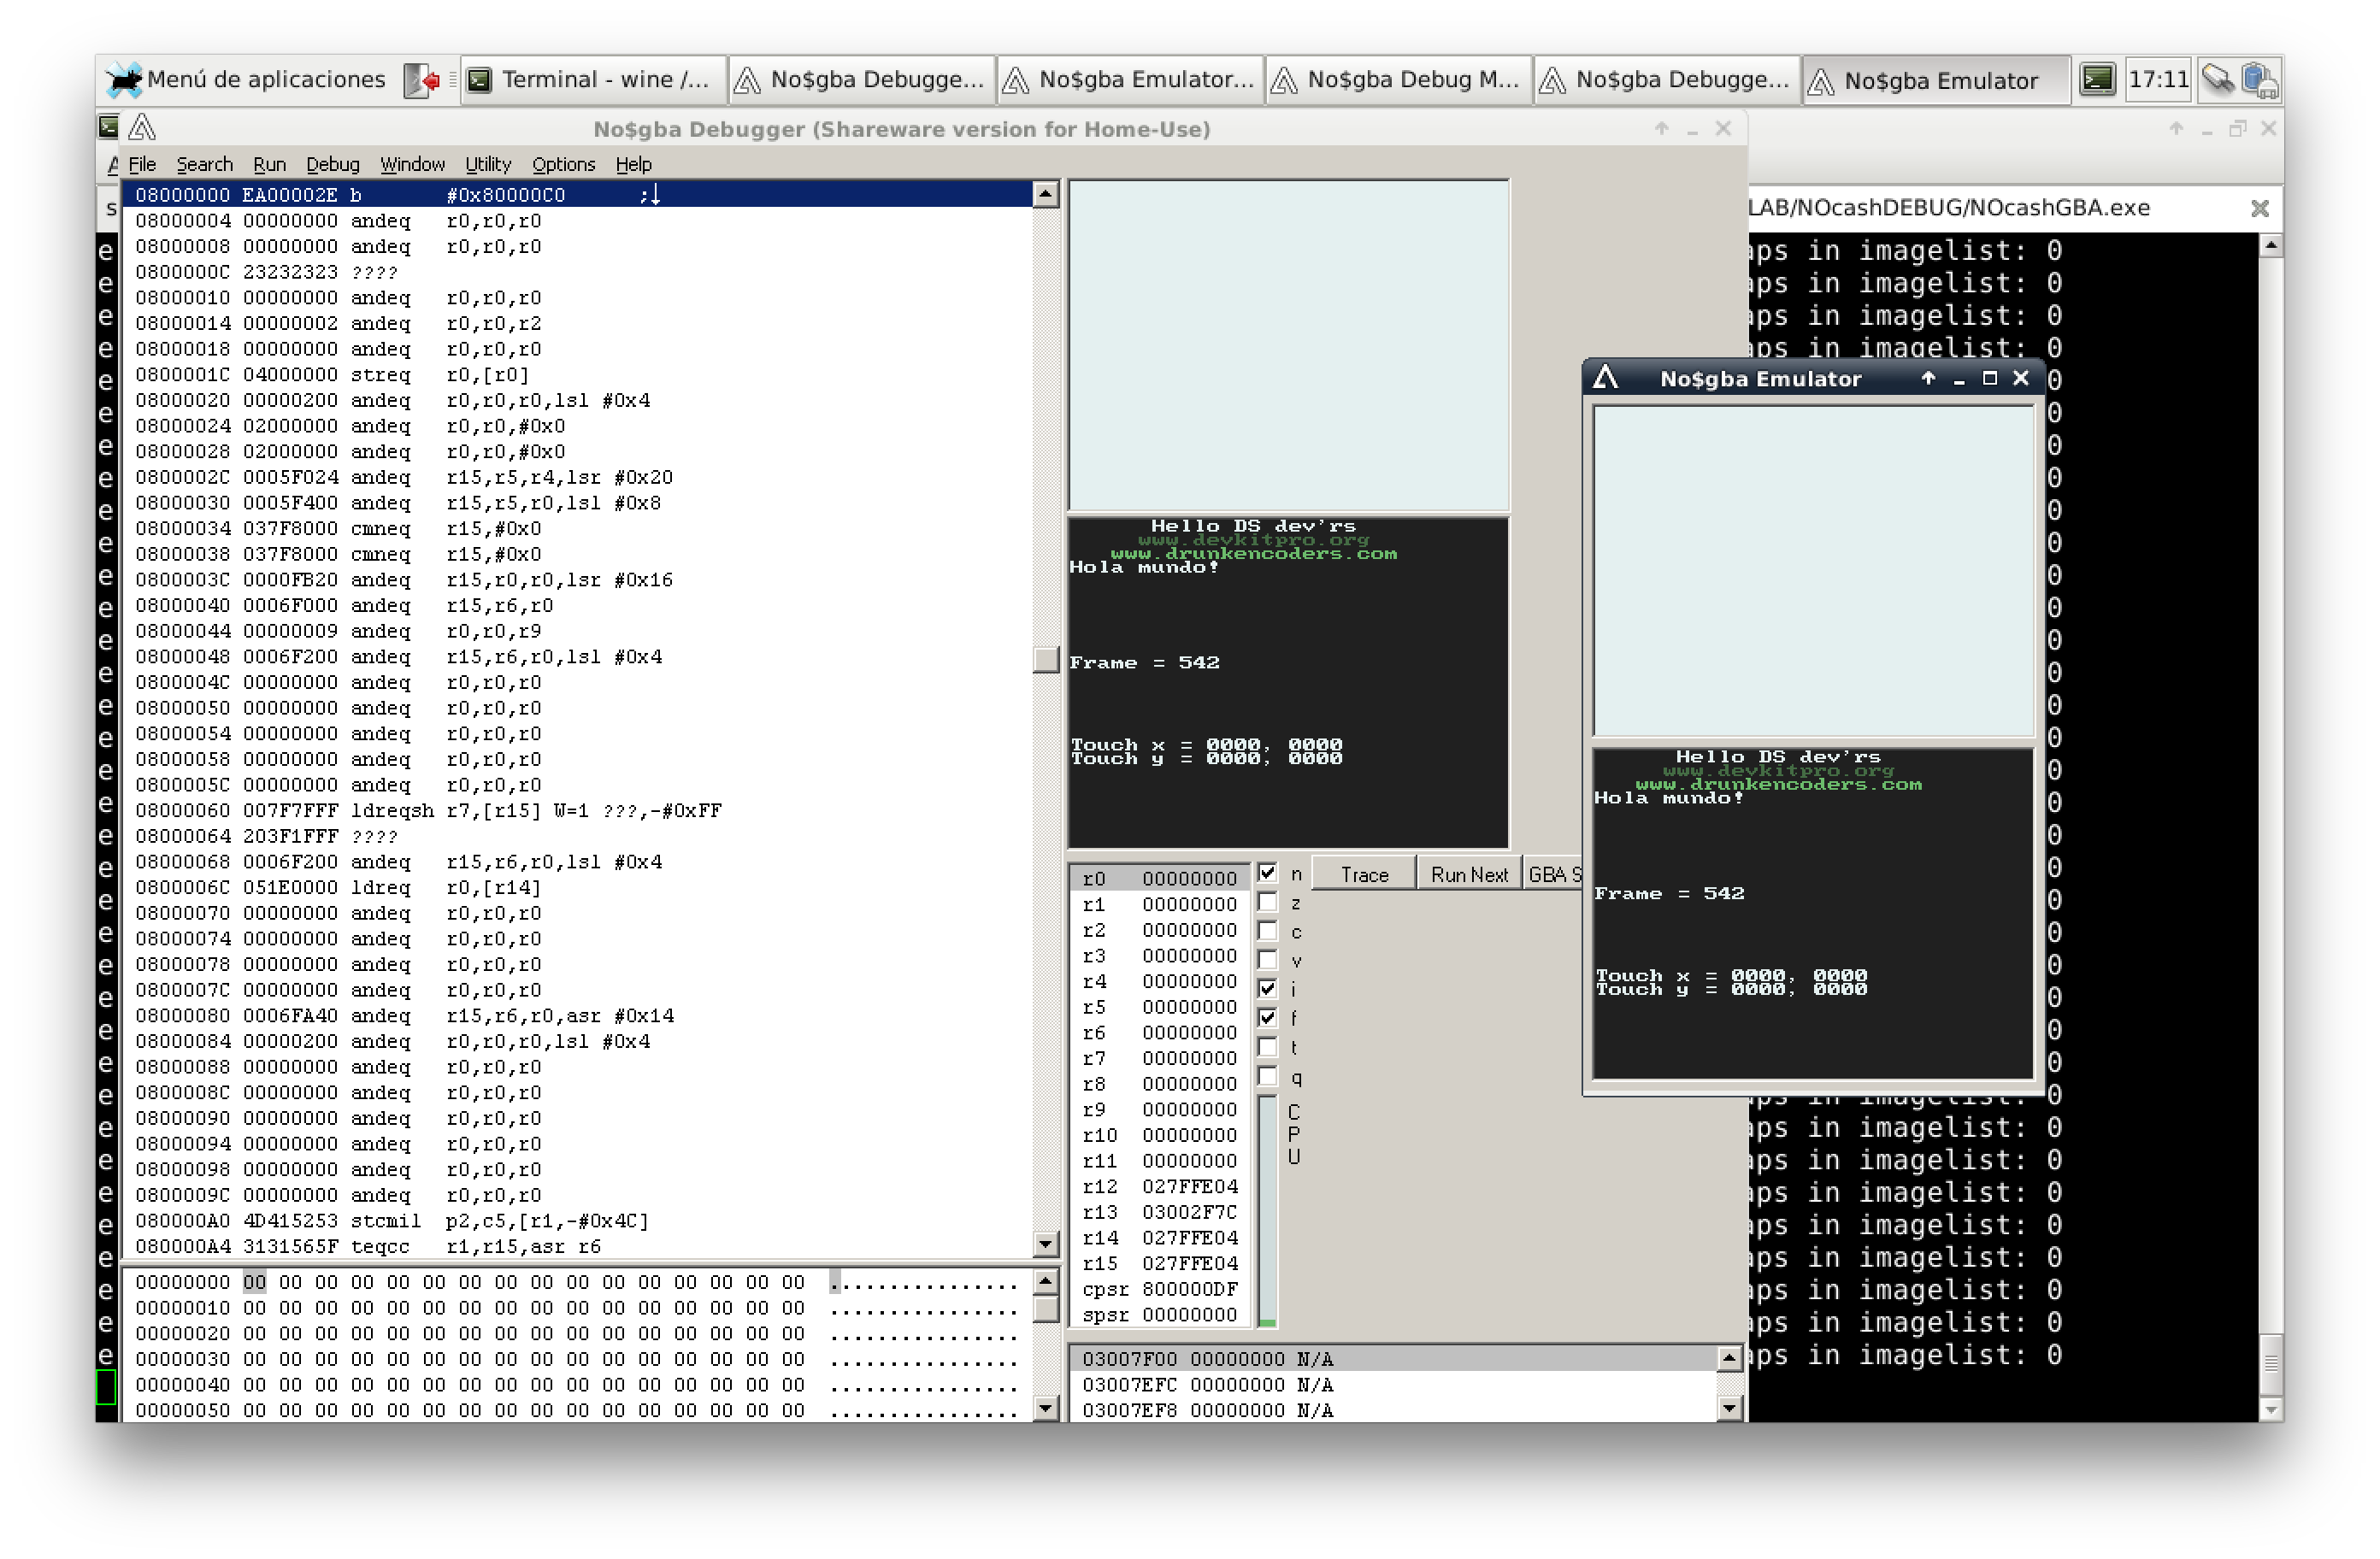
\includegraphics[width=0.95\textwidth]{P1Media/NoCashDebug}
\end{figure}
	
	\subsubsection{Ejecución de los proyectos de prueba sobre hardware real}
	
	Los programas desarrollados también se pueden ejecutar sobre hardware real mediante el uso de Flashcards para evitar el firmado de código. Las aplicaciones funcionan tanto en Nintendo DS como en Nintendo 2DS o 3DS gracias a la capa de compatibilidad que incluyen las consolas modernas de Nintendo.
	
\begin{figure}[h!]
	\caption{{\tt Hello World} ejecutado en una Nintendo 3DS.}
	\label{fig:dependency}
	\centering
	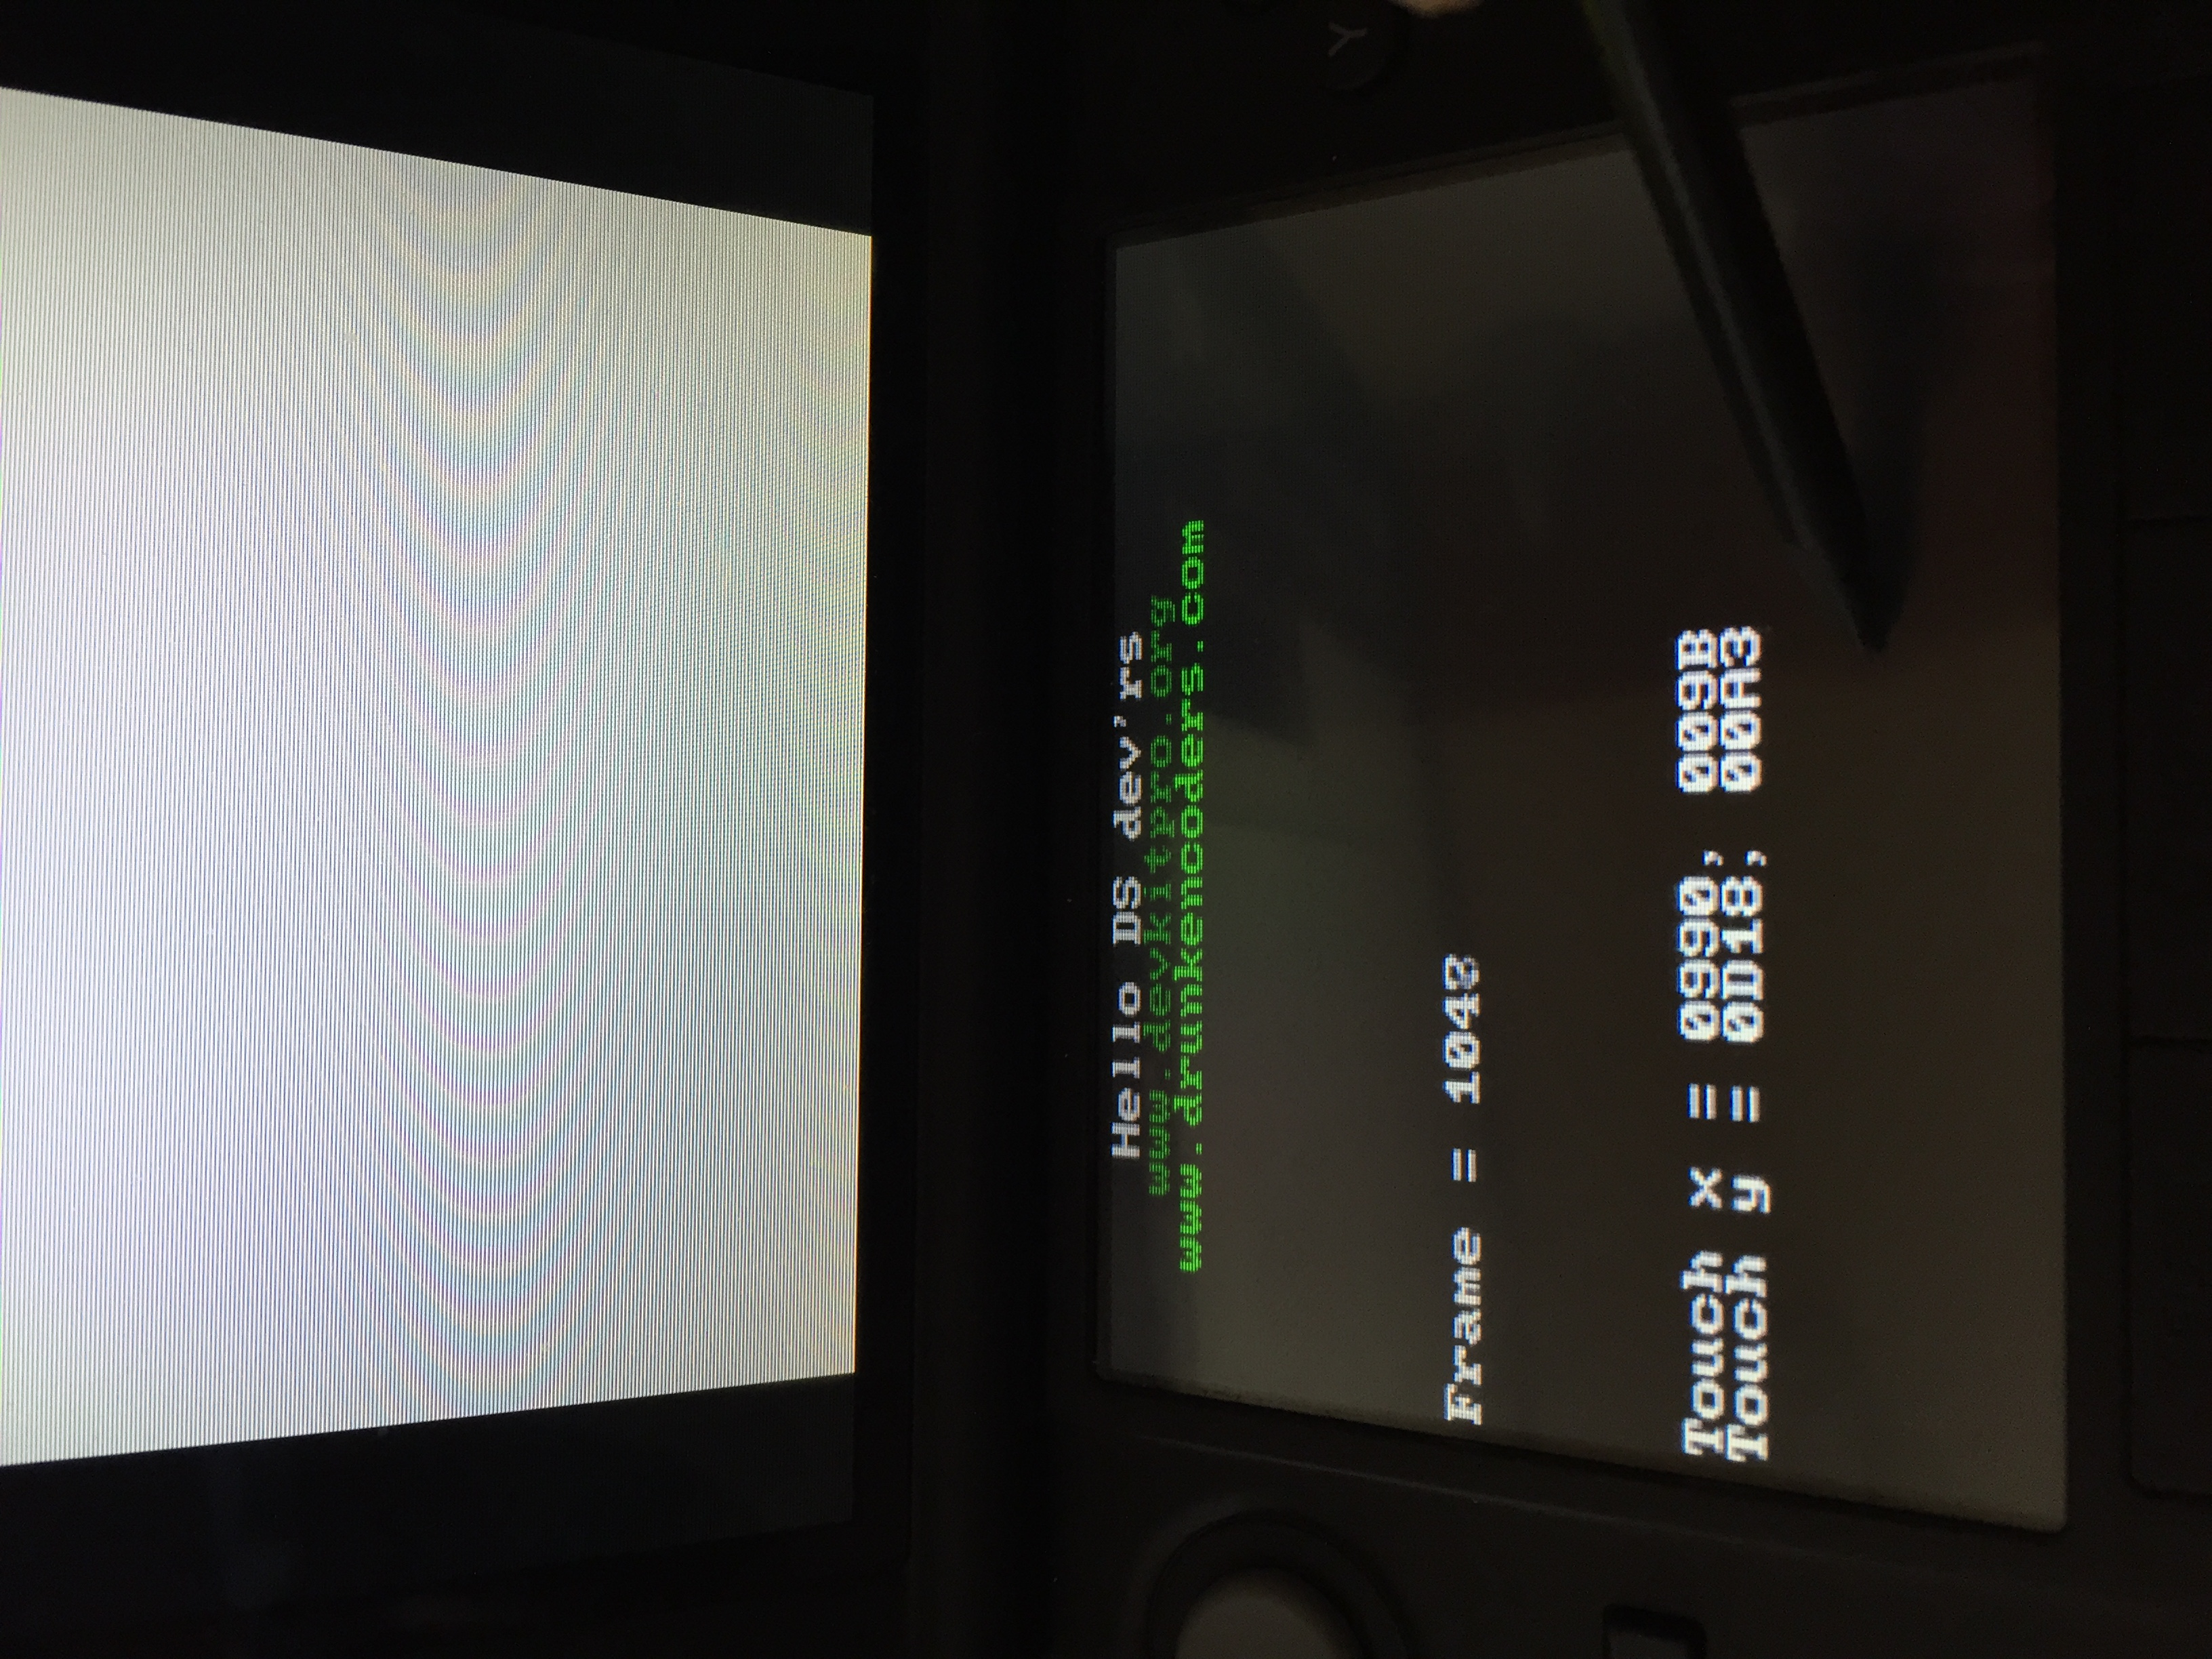
\includegraphics[width=0.95\textwidth,angle=270]{P1Media/3DS}
\end{figure}
	
	\subsection{Automatización de la instalación del entorno de desarrollo}
	
	Nuestro grupo trabaja sobre diversos sistemas operativos, como Mac OS X o Windows. Esta diversidad de software hace que sea realmente difícil aislar ciertos problemas dependientes del entorno de modo que resulta conveniente utilizar una máquina virtual a fin de evitar estos problemas de compatibilidad.
	
	Recurrimos a virtualizadores como VirtualBox o Parallels Desktop manejados mediante Vagrant para agilizar la puesta a punto del entorno, sin embargo en esta ocasión apostar por Vagrant no fue una buena decisión ya que nos encontramos con problemas a la hora de conseguir habilitar el entorno de escritorio por lo que finalmente instalamos Debian en la máquina virtual manualmente y aprovechamos el script que teníamos preparado para \emph{provisionar} la máquina para instalar todo el software necesario.
	
\begin{figure}
\lstinputlisting[basicstyle=\ttfamily\scriptsize,language=Ruby,frame=single]{../vagrant/Vagrantfile}
	\caption{Fichero {\tt Vagrantfile} de definición de la máquina virtual. Los archivos referidos en este fichero se corresponden con los fragmentos detallados en los apartados previos. El fichero {\tt personal.sh} únicamente instala {\tt vim} y {\tt zsh}.}
	\label{fig:Vagrantfile}
\end{figure}